\chapter[Gemeinsamkeiten und Unterschiede]{Gemeinsamkeiten und Unterschiede von SOA und Microservices}
\label{chap:Unterschiede}
%Einsatzmöglichkeiten!!!! 
% - nötigen Architekturen und Schnittstellen 
% - Plattformen und Voraussetzungen für den Einsatz der jeweiligen Paradigmen

%Vor- und Nachteile der Paradigmen, 
% - Prozessisolierung
% - Skalierung
% - Deployment
% - Wartbarkeit (insbesondere der Korrigierbarkeit, Erweiterbarkeit, Anpassbarkeit, Verbesserung)
% - Entwicklung/Testbarkeit 
% - Bindung an Technologiestacks
\section{Einsatzgebiet}
\label{sec:Einsatzgebiet}
Sowohl SOA, als auch das Microservice sind Paradigmen aus der Service-orientierten Architektur, verfolgen jedoch unterschiedliche Ansätze. Während das Microservice-Paradigma die Softwareentwicklungsabteilung unterstützen soll, soll mit Hilfe von SOA die Kommunikation zwischen den Anwendungen und den Abteilungen standardisiert und optimiert werden.
\\\\
Mit Hilfe des Microservice Paradigmas wird die Struktur einer Anwendung in mehrere, kleinere Dienste aufgeteilt. Dadurch ist es möglich neue Technologien einzusetzen und gegebenenfalls zu ersetzten, sollten diese nicht den gewünschten Erfolg bringen.
\\\\
Anders sieht es jedoch mit SOA aus. Hierbei werden Adapter für Anwendungen, wie ERP-, CRM- oder COBAL-Systeme, entwickelt, welche zusammen mit der Anwendung als Dienst dienen. Der Adapter stellt eine Schnittstelle für die Funktionalität der Anwendung bereit und übernimmt das steuern der Anwendung und das abfangen von Fehleingaben.

\section{Architekturen und Schnittstellen}
\label{sec:ArchitekturenUndSchnittstellen}
Beide Paradigmen sind Service-orientierte Systeme, dessen Grundlage ein verteiltes System ist. Dabei existieren eine beliebige Anzahl verschiedener Dienste, welche verschiedene Funktionalitäten bereitstellen. Damit der Ausfall eines Dienstes, keine weiteren Dienste direkt beeinflusst, werden diese oft in eigenen Umgebungen betrieben, wie Virtuelle Maschinen. Dies ist sowohl bei SOA, als auch bei Microservices der Fall, jedoch kann durch den Ausfall eines Dienstes die Kommunikation von anderen Diensten gestört werden.
\\\\
Während bei SOA eine zentrale Kommunikationseinheit (der ESB) existiert, sind Microservices in der Kommunikation frei. Dies bedeutet, dass der ESB in einem SOA-System entsprechende Werte oder Fehlermeldungen zurückgeben kann, während Microservices selber auf fehlgeschlagene Anfragen reagieren muss. Um dies zu verhindern, werden oft mehrere Instanzen eines kritischen Dienstes betrieben.
\\\\
Damit Dienste untereinander kommunizieren können, sind Schnittstellen (APIs) notwendig, über welche die Informationen abgefragt bzw. bereitgestellt werden können. Da jedoch in einem SOA-System ganze Applikationen wie CRM- oder COBOL-Systeme verwendet werden, ist es notwendig zunächst einmal zu entscheiden, wie dessen Funktionalitäten angeboten werden sollen.
\\\\
Zum einen können Adapter verwendet werden, die jegliche Informationen der Anwendung bereitstellen. Dadurch ist es möglich durch Standardisierte Verfahren wie SOAP/HTTP oder REST/HTTP den Dienst wiederzuverwenden. Jedoch muss dafür neben den Adaptern ein Integrations Hub (ESB) existieren, welche die Informationen verarbeiten und aufbereiten kann. 
\\\\
Zum anderen bedeutet diese Aufteilung, dass oft eine große Menge an Informationen abgefragt werden. Dies macht gegenüber dem Business kein Sinn, da zum Teil unnötig viele Informationen für die nächste Generation von Anwendungen bereitgestellt werden. In diesem Fall werden "`Service Komponenten"' verwendet, welche als Adapter dienen und die benötigten Informationen aus den Applikationen abfragen und bereitstellen.
\begin{figure}[htb]
    \centering 
    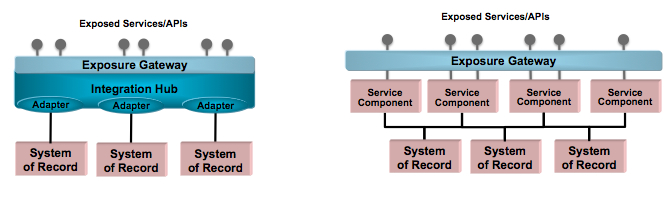
\includegraphics[width=\linewidth]{content/images/figure2}\
    \quelle\url{https://www.ibm.com/developerworks/websphere/library/techarticles/1601_clark-trs/1601_clark.html}
    \caption{Technische und Funktionale Sicht von SOA}
    \label{fig:TechnicalAndFunctionalViewsOfSOA} 
\end{figure}

Bei einem Microservice System stellt ein Microservice genau eine Fachlichkeit da und bietet diese über Schnittstellen an. Anders als bei SOA sind die Dienste deutlich kleiner, wodurch weniger Informationen bereitgestellt werden, je Microservice.
\begin{figure}[htb]
    \centering 
    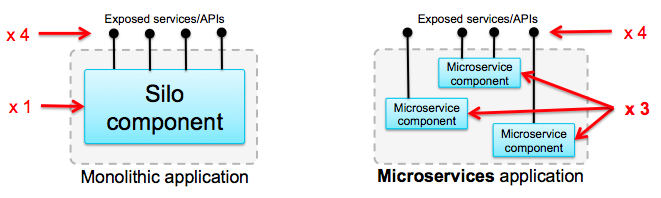
\includegraphics[width=\linewidth]{content/images/MonolithicVsMicroservice}\
    \quelle\url{https://www.ibm.com/developerworks/websphere/library/techarticles/1601_clark-trs/1601_clark.html}
    \caption{Monolithische vs Microservice Applikation}
    \label{fig:MonolithicVsMicroservice} 
\end{figure}
\newpage
Dies bedeutet jedoch auch, dass weitere Microservices notwendig sind, welche die Informationen von verschiedenen Microservices abfragen und zusammenfassen. Dadurch ergibt sich ein Geflecht aus Microservices, welche untereinander kommunizieren und zum Teil aufeinander angewiesen sind. Solange sich die Schnittstelle eines Dienstes nicht ändert, besteht kein Problem bei der Interoperabilität für das bestehende System. Erst wenn sich die Schnittstelle ändert und eine ältere Schnittstelle nicht mehr Angeboten wird, schadet dies der Interoperabilität.
\\\\
Dadurch, dass die Kommunikation über Schnittstellen erfolgt, kann, sofern diese Standardisiert sind und Beispielsweise als SOAP/HTTP oder REST/HTTP umgesetzt wurden, der Dienst Plattform unabhängig deployed werden. Da jedoch monolithische Anwendungen oft sehr umfangreich sind, werden diese meistens für ein bestimmtes Betriebssystem gebaut. Microservices hingegen sind kleine autarke Dienste, Dadurch ist es möglich diese Plattform unabhängig zu deployen. Hier drauf wird in weiter unten, unter \ref{subsec:BindungAnTechnologiestacks} \nameref{subsec:BindungAnTechnologiestacks}, genauer eingegangen.

\section{Vor- und Nachteile}
\label{sec:VorUndNachteile}

\subsection{Prozessisolierung}
\label{subsec:Prozessisiolierung}
Ein wichtiger Grundsatz von Service-orientierten Systemen ist, dass Dienste autark bleiben. Um dies zu erreichen, darf nur eine lose Kopplung zwischen einzelne Dienste stattfinden. Dies wird durch Zustandslose Schnittstellen und Eigenständigkeit erreicht. Damit ist gemeint, dass jeder Dienst seine Aufgaben, zum größten Teil alleine durchführen kann ohne auf andere Dienste angewiesen zu sein.
\\\\
Eine Vollständige Autarkheit ist in einem Microservice System nicht möglich, da ein vollständiges Microservice System die Abbildung einer Applikation ist. Dabei wurden einzelne Fachlichkeiten in Microservices verpackt. Dadurch können einige Microservices nicht lose gekoppelt sein, sondern benötigen weitere Microservices.

\begin{figure}[htb]
    \centering 
    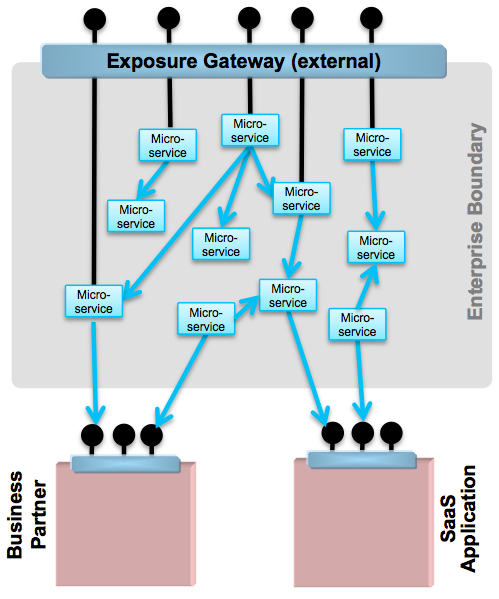
\includegraphics[width=300px]{content/images/figure6}\
    \quelle\url{https://www.ibm.com/developerworks/websphere/library/techarticles/1601_clark-trs/1601_clark.html}
    \caption{Microservice Architektur}
    \label{fig:MicroserviceArchitekturInGreenField} 
\end{figure}
\newpage
Bei SOA hingegen besteht ein Dienst, wie bereits in \ref{sec:UnternehmensKomponenten} \nameref{sec:UnternehmensKomponenten} erwähnt, aus einer vollständigen Anwendung und einem Adapter, welcher die Steuerung der Anwendung über APIs bereitstellt. Dadurch dass eine Anwendung alle nötigen Fachlichkeiten und Ressourcen, für die Ausführung der Anwendung besitzt, ist der Dienst vollständig Autark. Lediglich die Frontend-Anwendungen sind auf die APIs und damit auf die Backend-Anwendungen angewiesen. Fällt zum Beispiel eine Anwendung aus, kann es dazu führen, dass das gesamte System nicht mehr funktioniert, da die Dienste häufig in eine Wertschöpfungskette eingebunden sind.

\subsection{Deployment}
\label{subsec:Deployment}
Das Deployment ist in einem Service-orientiertem System von entscheidender Bedeutung und darf nicht unterschätzt werden. Oft werden Continuous Deployment Pipelines aufgebaut, um diesen Prozess zu automatisieren. Innerhalb der Pipeline wird sowohl die Umgebung, in welcher der Dienst später laufen soll, aufgebaut, sowie der Dienst in die zuvor, vorbereitete Umgebung deployed. Unter Umständen ist ein erneutes Deployen notwendig, wenn sich die Anforderungen an einen Dienst geändert haben oder Fehler behoben wurden. Dabei stellt das Deployment eine besondere Herausforderung dar. Hauptproblem ist die nötigen Abhängigkeiten, für die Ausführung der Dienste, bereitzustellen und die nötigen Konfigurationen vorzunehmen.
\\\\
Dadurch, dass Microservices kleine autarke Dienste sind, ist es oft nicht nötig, viele Konfigurationsdateien anzupassen bzw. bereitzustellen. Jedoch sind oft eine Vielzahl von Microservices in einem System vorhanden und müssen deployed, sowie gemanagt werden. Durch Werkzeuge wie \gls{glos:Docker} und \gls{glos:Vagrant} wird das Deployment zusätzlich vereinfacht. 
\\\\
Dienste in einem SOA-System hingegen sind häufig ganze Anwendungen. Diese erfordern oft eine aufwändige Konfiguration, welche nicht immer mit Hilfe von Konfigurationsdateien vorgenommen werden können. Einige Anwendungen dürfen nur durch den Hersteller oder durch ihn Zertifizierte Unternehmen Installiert und/oder Konfiguriert werden. Dadurch ist ein automatisches Deployment nicht möglich und auch ein manuelles Deployment wird erschwert.
\\\\
Im Rahmen einer Wartung müssen Dienste, oft erneut ausgeliefert werden, um Fehler zu beheben oder ihn anzupassen. In diesem Falle existieren in der Regel die Umgebungen, für den Einsatz des Dienstes. Jedoch müssen diese gegebenenfalls angepasst werden. Die ist in einem Microservice-System durch Werkzeuge wie Docker ebenfalls standardisiert. In einem SOA-System hingegen muss dies oft manuell durchgeführt werden.

\subsection{Skalierung}
\label{subsec:Skalierung}
Nicht immer können stark genutzte Anwendungen, durch Aufwertung oder Erweiterung von Hardware, belastbarer gemacht werden. Kritische oder Zentrale Anwendungen eines Unternehmens sind nicht nur stark genutzt, sondern dürfen nicht ausfallen. Durch Hardware, kann nicht durchgängig sichergestellt werden, dass eine Anwendung erreichbar ist. Um diese Problematiken entgegen zu wirken, muss Skaliert werden. Dabei werden mehrere Instanzen eines Systems parallel betrieben.
\\\\
In einem Microservice-System, ist durch das vereinfachte Deployment möglich, in kürzester Zeit eine weitere Instanz eines Dienstes zu starten und zu betreiben. Dies kann durch einen Standardisierten Deployment Prozess automatisiert werden. Dadurch kann in kürzester Zeit auf verschiedene Lasten von Diensten reagiert werden, ohne dass ein Mensch in das System eingreifen muss. Es ist bei einem Microservice-System möglich, wenig genutzte Dienste, nur bei bedarf zu starten und nach einer gewissen Zeit der Inaktivität, zu stoppen. Kritische oder stark genutzte Dienste hingegen, besitzen meistens mehrere Instanzen, auf denen die Lasten verteilt werden. Dadurch wird ebenfalls eine Ausfallsicherheit gewährleistet.
\\\\
SOA-Systeme besitzen deutlich größere Dienste als Microservice-Systeme. Dadurch dass, wie bereits unter \ref{subsec:Deployment} \nameref{subsec:Deployment} erwähnt, der Deployment Prozess nicht Standardisiert ist, ist ein einfaches, automatisches Skalieren nicht möglich. Das Skalieren eines Dienstes kann dementsprechend, nur manuell geschehen und ist oft mit viel Aufwand verbunden. Muss ein Dienst dennoch mehrere Instanzen besitzen, so werden diese meistens dauerhaft, parallel betrieben.
\\\\
Viele monolithische Anwendungen sind zudem nicht Zustandslos, wodurch ein Skalieren zusätzlich erschwert wird. Microservices hingegen müssen so erstellt werden, dass sie Zustandslos sind, da ein Dienst nicht sicherstellen kann, dass die Anfragen vom gleichen Dienst oder Benutzer stammen.

\subsection{Wartbarkeit}
\label{subsec:Wartbarkeit}
Im laufe der Zeit wachsen die Anforderungen an einen Dienst, wodurch dieser angepasst, verbessert oder erweitert werden muss. Zur Wartung gehört jedoch auch das korrigieren von Fehlern, welches einer der einfachsten Aufgaben in einem Service-orientierten System ist, da sich dadurch meistens, nicht die Schnittstellen, Umgebung oder die Konfiguration des Dienstes ändert. Anders sieht dies jedoch beim anpassen, verbessern oder erweitern aus.
\\\\
Das Anpassen einer Anwendung kann sich von dem Verbessern oder Erweitern einer Anwendung unterscheiden. Zum Beispiel reicht es aus die Mehrwertsteuer in einer Anwendung zu ändern, welches eine Anpassung darstellt, jedoch keine Verbesserung oder Erweiterung. Das Anpassen ist durch die kaum veränderten Strukturen relativ leicht. Anders sieht dies jedoch bei Verbesserungen oder Erweiterungen aus. Beide Änderungen sorgen für eine Veränderung der internen Struktur des Quelltextes. Zusätzlich ist man an den vorgegebenen Technologiestacks gebunden. Oft sind Verbesserungen oder Erweiterungen nicht ohne das Verändern der Quelltextstruktur möglich.
\\\\
Während in einem SOA-System der Dienst aus einer Anwendung und einem Adapter besteht und damit ein fast monolithisches System abbildet. Besteht ein Microservice-System aus viele unterschiedlichen Diensten. In beiden Systemen ist es möglich, in kürzester Zeit Fehler zu korrigieren, sofern die nötigen Voraussetzungen gegeben sind. Das Anpassen, Verbessern oder Erweitern eines Dienstes, gestaltet sich jedoch einfacher in einem Microservice-System, als in einem SOA-System. Aufgrund der Größe von Microservices, kann ein Microservice von Grund auf neu erstellt werden, sollte dies nötig sein. Muss das System erweitert werden, können neue Microservices erstellt, welche die neuen Anforderungen bzw. Fachlichkeiten abbilden. Durch die Autarkheit von Microservices, können diese deployet werden, ohne die Interoperabilität des bestehenden Systems zu gefährden oder zu beeinflussen. Anschließend müssen gegebenenfalls einzelne Dienste angepasst werden, um die neuen Funktionalitäten, in das bestehende System, einzubinden.

\subsection{Bindung an Technologiestacks}
\label{subsec:BindungAnTechnologiestacks}
In beiden Paradigmen, sollten Dienste eine standardisierte Schnittstelle besitzen, damit diese, durch andere Dienste verwendet werden können. Zusätzlich ist dadurch eine Wiederverwendung des Dienstes möglich. Das verwenden einer standardisierten Schnittstelle schränkt jedoch die Auswahl der einzusetzenden Technologien ein. Zudem ist das verwenden einer standardisierten Schnittstelle nicht immer möglich.
\\\\
In einem Microservice-System ist die Wiederverwendbarkeit ein wichtiges Thema. Dadurch wird man gezwungen, die Schnittstellen zu standardisieren. Oft werden hierfür REST-HTTP Schnittstellen, welche Sprachen unabhängig sind, verwendet. REST-HTTP basiert dabei auf dem HTTP-Protokoll. Dadurch kann die Schnittstelle in fast jeder Programmiersprache verwendet werden, wodurch ein Dienst ebenfalls in fast jeder Programmiersprache geschrieben werden kann. Durch die Größe eines Microservices ist es ebenfalls möglich, neue Technologien zu Testen und in der Produktion einzusetzen. Dabei können verschiedenen Sprachen, sowie Frameworks verwendet werden, um die Aufgabe zu erledigen. Stellt sich heraus, dass eine Technologie, Sprache oder Framework sich nicht für die Erledigung einer Aufgabe eignet, kann der Dienst, aufgrund seiner Größe, in kürzester Zeit ausgetauscht werden. Jedoch birgt das einsetzten neuer Technologien auch Gefahren. So ist die Versuchung Groß, experimentelle oder ungetestete Technologien in Produktion einzusetzen, ohne zuvor zu Testen, welche Auswirkungen die Technologie auf das System hat.
\\\\
Ein Dienst in einem SOA-System beinhaltet eine monolithische Anwendung. Die Schnittstellen werden durch Adapter bereitgestellt. Diese müssen mit der Anwendung interagieren können, wodurch der Adapter oft in der selben Sprache geschrieben werden muss, wie die zu interagierenden Anwendung. Aufgrund der Größe von Monolithen ist es nicht möglich, diese in kürzester Zeit auszuwechseln. Zudem muss man sich bei der Entwicklung einer Anwendung, auf einen Technologiestack festlegen. Dadurch ist man bei der Weiterentwicklung oder Wartung der Anwendung an diesen gebunden. Eine neue Technologie einzuführen, würde bedeuten die Struktur der Anwendung zu verändern.

\subsection{Entwicklung und Testbarkeit}
\label{subsec:EntwicklungUndTestbarkeit}
Damit ein Dienst in die jeweiligen Systeme eingebunden werden kann, muss dieser zunächst entwickelt und getestet werden. Dabei ist zu beachten, dass in einem SOA-System, ein Dienst eine monolithische Anwendung mit Adapter ist, während ein Microservice-System eine vollständige Anwendung beschreibt und ein Dienst nur ein Teil der Anwendung ist.
\\\\
Durch diese Unterschiede ist nicht nur die Größe des Entwicklerteams unterschiedlich, sondern auch der Entwicklungsprozess. In einem Microservice-System werden häufig DevOp-Teams in der Größe von 4-6 Personen eingesetzt. Da ein Dienst in einem Microservice-System, nur von einem Team entwickelt werden sollte, stellt dies eine Begrenzung der Größe eines Dienstes dar. Dadurch ist in der Regel ein Microservice deutlich kleiner, als eine monolithische Anwendung, jedoch nicht immer einfacher zu entwickeln.
\\\\
Während bei einer monolithischen Anwendung, alle nötigen Abhängigkeiten in einem Projekt vorhanden sind, muss bei Microservices dafür gesorgt werden, dass die Abhängigkeiten korrekt aufgelöst werden, da diese in dem Bereich anderer Microservices  liegen. Damit die Abhängigkeiten korrekt aufgelöst werden können, muss ein Entwickler wissen, welche Abhängigkeiten die korrektens ind.. In einem Microservice-System gibt es eine sehr große Menge an Diensten, welche verschiedene Fachlichkeiten bereitstellen, daher ist es nicht immer einfach den richtigen Service auszuwählen.
\\\\
Nach der Entwicklung eines Dienstes, muss dieser getestet werden, bevor der Dienst in die Produktion deployed werden kann. In einer monolithischen Anwendung, kann mit Hilfe von automatischen JUnit Tests ein Großteil der Funktionalität getestet werden. Es kann unter anderem getestet werden, ob jegliche Abhängigkeiten innerhalb der Anwendung einwandfrei funktionieren. Benötigt ein Microservice keine anderen Dienste, so kann mit Hilfe von JUnit Tests ebenfalls die Funktionalität vollständig geprüft werden. Anders sieht das jedoch bei Microservices aus, die auf weitere Dienste angewiesen sind. Hierbei müssen entweder die anderen Dienste simuliert werden oder der Microservice muss in eine entsprechende Testumgebung deployed und dort getestet werden. Das betreiben einer solchen Testumgebung ist nicht unproblematisch, da eine exakte Kopie des Produktivsystems notwendig ist, um relevante Testergebnisse zu erlangen.
\\\\
Zudem sollte in jedem der beiden Systeme getestet werden, wie sich einzelne Services, beziehungsweise das gesamte System, bei zufälligen Ausfällen von verschiedenen Systemen, verhalten. Dies stellt eine besondere Herausforderung dar, da dies meistens nur in der Produktionsumgebung möglich ist. Netflix Inc., welches auf Microservices für ihren Dienst "`Netflix"' setzt, hat für diesen Zweck ein Werkzeug Namens "`chaosmonkey"' entwickelt, welches willkürlich Systeme innerhalb seines Dienstes "`Netflix"' abschaltet.\footnote{\cite{chaosmonkey}}
